\section{Pipelining}
\label{sec:pipelining}
\sources{Lecture ``Pipelining'' (\nolinkurl{03-pipelining-lecture.pdf}); H\&P 5th
ed.\ App.~C (Pipelining: Basic and Intermediate Concepts).}

\subsection{What Is Pipelining?}
\label{sec:pipelining-idea}

\begin{definition}[Pipelining]
\textbf{Pipelining} is an implementation technique in which multiple
instructions are overlapped in execution.\HPA{C}{\S C.1}{2}
\end{definition}

Real-life pipelining examples:
\begin{itemize}
  \item Doing laundry (washing, drying, folding multiple loads)
  \item Factory production lines
  \item Traffic (?)
\end{itemize}

\subsubsection{Instruction Pipelining}

\begin{definition}[Instruction pipeline, stage, machine cycle]
\leavevmode
\begin{itemize}
  \item Instruction pipelining is a CPU implementation technique where
  \textbf{multiple operations} on a number of instructions are \textbf{overlapped}.
  \item An instruction execution pipeline involves a number of steps, where each
  step completes a part of an instruction. Each step is called a \emph{pipeline
  stage} or \emph{pipeline segment}.
  \item The stages are connected in a \textbf{linear fashion}: one stage to the
  next, forming the pipeline -- instructions enter at one end, progress through
  the stages, and exit at the other end.
  \item The time to move an instruction one step down the pipeline is equal to
  \emph{the machine cycle} and is determined by the stage with the longest
  processing delay.
\end{itemize}\HPA[10]{C}{\S C.1, The Classic Five-Stage Pipeline}{6}
\end{definition}

\begin{itemize}
  \item Pipelining \textbf{increases} the CPU \textbf{instruction throughput}:
  the number of instructions completed per cycle.
  \begin{itemize}
    \item Under ideal conditions (no stall cycles), instruction throughput is
    one instruction per machine cycle, i.e.\ \textcolor{red}{ideal CPI = 1}.
  \end{itemize}
  \item Pipelining \textbf{does not reduce} the execution time of an
  individual instruction: the time needed to complete all processing steps of
  an instruction (also called \emph{instruction completion latency}).
  \begin{itemize}
    \item Minimum instruction latency $= n$ cycles, where $n$ is the number of
    pipeline stages.
  \end{itemize}
\end{itemize}

\begin{explanation}
\textbf{Why is the ideal CPI equal to 1?} CPI counts how many cycles pass, on
average, between \emph{completions} of instructions -- not how long each
instruction takes. In a $k$-stage pipeline each instruction still needs $k$
cycles from fetch to write-back, but once the pipeline is full a new
instruction enters and an old one leaves every cycle. For $n$ instructions the
pipeline needs $k + (n-1)$ cycles, so
\[
  \CPI = \frac{k + n - 1}{n} \;\longrightarrow\; 1 \quad (n\to\infty).
\]
The fill cost of $k-1$ cycles is paid only once. Stalls caused by hazards add
cycles without completing instructions, which is why real pipelines have
$\CPI = 1 + \text{stall cycles per instruction}$.
\end{explanation}

\subsection{Pipelining Example: Laundry}
\label{sec:laundry}

\begin{eg}[Doing laundry]
Ann, Brian, Cathy, and Dave (A, B, C, D) each have one load of clothes to
wash, dry, and fold.
\begin{itemize}
  \item Washer takes 30 minutes
  \item Dryer takes 40 minutes
  \item ``Folder'' takes 20 minutes
\end{itemize}
\end{eg}

\subsubsection{Sequential laundry}

\begin{center}\begin{minipage}{\linewidth}\centering
\begin{tikzpicture}[x=0.95cm,y=-0.9cm,font=\scriptsize]
  \draw[-{Stealth}] (0,-0.6) -- (12.4,-0.6) node[right] {time (hours)};
  \foreach \t/\lab in {0/6PM,1.5/7,3.5/8,5.5/9,7.5/10,9.5/11,11.5/Midnight}
    \node at (\t,-1.0) {\lab};
  \foreach \task/\row in {A/0,B/1,C/2,D/3}{
    \pgfmathsetmacro{\xoff}{\row*3}
    \node[left] at (-0.3,\row) {\task};
    \draw[fill=white]    (\xoff,\row-0.35) rectangle ++(1,0.7) node[midway]{Wash};
    \draw[fill=black!12] (\xoff+1,\row-0.35) rectangle ++(1.33,0.7) node[midway]{Dry};
    \draw[fill=black!28] (\xoff+2.33,\row-0.35) rectangle ++(0.67,0.7) node[midway]{Fold};
  }
\end{tikzpicture}
\diagramsource{\nolinkurl{03-pipelining-lecture.pdf}, slide 6 (``Sequential Laundry'')}
\end{minipage}
\end{center}

\begin{remark}
\textbf{Sequential laundry takes 6 hours for 4 loads} (each load: $30+40+20=90$
min, done strictly one after another).
\end{remark}

\subsubsection{Pipelined laundry (start work ASAP)}

\begin{center}\begin{minipage}{\linewidth}\centering
\begin{tikzpicture}[x=1.05cm,y=-0.9cm,font=\scriptsize]
  \draw[-{Stealth}] (0,-0.6) -- (7.2,-0.6) node[right]{time (hours)};
  \foreach \t/\lab in {0/6PM,1.5/7,3.5/8,5.5/9}
    \node at (\t,-1.0) {\lab};
  \foreach \task/\row in {A/0,B/1,C/2,D/3}{
    \pgfmathsetmacro{\xoff}{\row*1.33}
    \node[left] at (-0.3,\row) {\task};
    \draw[fill=white] (\xoff,\row-0.35) rectangle ++(1,0.7) node[midway]{Wash};
    \draw[fill=black!12]   (\xoff+1,\row-0.35) rectangle ++(1.33,0.7) node[midway]{Dry};
    \draw[fill=black!28]    (\xoff+2.33,\row-0.35) rectangle ++(0.67,0.7) node[midway]{Fold};
  }
\end{tikzpicture}
\diagramsource{\nolinkurl{03-pipelining-lecture.pdf}, slide 7 (``Pipelined Laundry Start work ASAP'')}
\end{minipage}
\end{center}

\begin{remark}
\textbf{Pipelined laundry takes 3.5 hours for 4 loads.}
\[
  \text{Speedup} = \frac{6}{3.5} = 1.7
\]
\end{remark}

\subsubsection{Pipelining lessons}

\begin{noot}{Pipelining lessons}
\begin{itemize}
  \item Pipelining does not help the \textbf{latency} of a single task; it
  helps the \textbf{throughput} of the entire workload.
  \item Pipeline rate is limited by the \textbf{slowest} pipeline stage.
  \item Multiple tasks operate \textbf{simultaneously}, using
  \textbf{different resources}.
  \item Potential speedup $=$ number of pipe stages.
  \item Unbalanced lengths of pipe stages reduce speedup (dryer is the
  bottleneck at 40 min $\Rightarrow$ every stage effectively takes 40 min).
  \item Time to ``fill'' the pipeline and time to ``drain'' it reduces
  speedup.
  \item As long as we have \textbf{separate resources}, we can pipeline the
  tasks.
  \item If one load depends on another, we have to wait (delay/stall for
  \emph{dependencies}).
\end{itemize}
\end{noot}

\subsection{CPU Pipelining}
\label{sec:cpu-pipelining}

\subsubsection{The 5 classic MIPS stages}

\begin{enumerate}
  \item \textbf{IF} -- Fetch instruction from instruction memory
  \item \textbf{ID} -- Read registers while decoding the instruction
  (Reg/Dec)
  \item \textbf{EX} -- Execute the operation or calculate an address,
  depending on instruction type
  \item \textbf{MEM} -- Access an operand from data memory
  \item \textbf{WB} -- Write the result into a register
\end{enumerate}

\begin{center}\begin{minipage}{\linewidth}\centering
\begin{tikzpicture}[font=\small]
  \draw[-{Stealth}] (0,0) -- (8.2,0);
  \foreach \x/\lab in {0.8/Cycle 1,2.4/Cycle 2,4.0/Cycle 3,5.6/Cycle 4,7.2/Cycle 5}
    \node[above] at (\x,0.15) {\lab};
  \node[left] at (-0.3,-0.6) {Load};
  \foreach \x/\lab in {0/Ifetch,1.6/Reg/Dec,3.2/Exec,4.8/Mem,6.4/Wr}
    \draw[fill=black!8] (\x,-1.0) rectangle ++(1.5,0.7) node[midway]{\scriptsize \lab};
\end{tikzpicture}
\diagramsource{\nolinkurl{03-pipelining-lecture.pdf}, slide 12 (``CPU Pipelining'') (resources for a load)}
\end{minipage}
\end{center}

Resources needed by a \texttt{lw} (load) instruction at each stage:

\begin{center}
\begin{tabular}{@{}ll@{}}
\toprule
Stage & Resource \\
\midrule
Ifetch (IF)  & Instruction memory (IM) \\
Reg/Dec (ID) & Register file \& decoder (Reg) \\
Exec (EX)    & ALU \\
Mem (MEM)    & Data memory (DM) \\
Wr (WB)      & Register file (Reg) \\
\bottomrule
\end{tabular}
\end{center}

\begin{note}
Accessing source and destination registers happens in \emph{two different
halves} of the clock cycle:
\begin{itemize}
  \item \textbf{Read} occurs in the 2\textsuperscript{nd} half of the ID
  cycle.
  \item \textbf{Write} occurs in the 1\textsuperscript{st} half of the WB
  cycle.
\end{itemize}
This lets an instruction read a register in the same cycle that an earlier
instruction writes it, and get the correctly updated value.
\end{note}

\subsubsection{Single-cycle vs.\ pipelined execution -- example}

Consider three loads: \texttt{lw \$1,100(\$0)}, \texttt{lw \$2,200(\$0)},
\texttt{lw \$3,300(\$0)}. Each of the 5 stages below is 2\,ns (limited by the
slowest resource); a non-pipelined machine needs one long 8\,ns cycle per
instruction.

\textbf{Single-cycle, non-pipelined:} total time for 3 instructions
$= 3 \times 8\text{ns} = 24$\,ns.

\begin{center}\begin{minipage}{\linewidth}\centering
\begin{tikzpicture}[x=0.51cm,y=1cm,font=\scriptsize]
  \draw[-{Stealth}] (0,0.6) -- (24.6,0.6) node[right] {ns};
  \draw (0,0.55) -- (0,0.65) node[above,font=\tiny] {0};
  \draw (2,0.55) -- (2,0.65) node[above,font=\tiny] {2};
  \draw (4,0.55) -- (4,0.65) node[above,font=\tiny] {4};
  \draw (6,0.55) -- (6,0.65) node[above,font=\tiny] {6};
  \draw (8,0.55) -- (8,0.65) node[above,font=\tiny] {8};
  \draw (10,0.55) -- (10,0.65) node[above,font=\tiny] {10};
  \draw (12,0.55) -- (12,0.65) node[above,font=\tiny] {12};
  \draw (14,0.55) -- (14,0.65) node[above,font=\tiny] {14};
  \draw (16,0.55) -- (16,0.65) node[above,font=\tiny] {16};
  \draw (18,0.55) -- (18,0.65) node[above,font=\tiny] {18};
  \draw (20,0.55) -- (20,0.65) node[above,font=\tiny] {20};
  \draw (22,0.55) -- (22,0.65) node[above,font=\tiny] {22};
  \draw (24,0.55) -- (24,0.65) node[above,font=\tiny] {24};
  \node[anchor=east] at (-0.3,-0.00) {\texttt{lw \$1,100(\$0)}};
  \draw (0,-0.270) rectangle (2,0.270) node[midway,font=\scriptsize] {Fetch};
  \draw (2,-0.270) rectangle (3,0.270) node[midway,font=\tiny] {Reg};
  \draw (3,-0.270) rectangle (5,0.270) node[midway,font=\scriptsize] {ALU};
  \draw (5,-0.270) rectangle (7,0.270) node[midway,font=\scriptsize] {Data};
  \draw (7,-0.270) rectangle (8,0.270) node[midway,font=\tiny] {Reg};
  \draw[{Latex[length=1.5mm]}-{Latex[length=1.5mm]}] (0,-0.38) -- (8,-0.38) node[midway,below,font=\tiny] {8 ns};
  \node[anchor=east] at (-0.3,-1.10) {\texttt{lw \$2,200(\$0)}};
  \draw (8,-1.370) rectangle (10,-0.830) node[midway,font=\scriptsize] {Fetch};
  \draw (10,-1.370) rectangle (11,-0.830) node[midway,font=\tiny] {Reg};
  \draw (11,-1.370) rectangle (13,-0.830) node[midway,font=\scriptsize] {ALU};
  \draw (13,-1.370) rectangle (15,-0.830) node[midway,font=\scriptsize] {Data};
  \draw (15,-1.370) rectangle (16,-0.830) node[midway,font=\tiny] {Reg};
  \draw[{Latex[length=1.5mm]}-{Latex[length=1.5mm]}] (8,-1.48) -- (16,-1.48) node[midway,below,font=\tiny] {8 ns};
  \node[anchor=east] at (-0.3,-2.20) {\texttt{lw \$3,300(\$0)}};
  \draw (16,-2.470) rectangle (18,-1.930) node[midway,font=\scriptsize] {Fetch};
  \draw (18,-2.470) rectangle (19,-1.930) node[midway,font=\tiny] {Reg};
  \draw (19,-2.470) rectangle (21,-1.930) node[midway,font=\scriptsize] {ALU};
  \draw (21,-2.470) rectangle (23,-1.930) node[midway,font=\scriptsize] {Data};
  \draw (23,-2.470) rectangle (24,-1.930) node[midway,font=\tiny] {Reg};
  \draw[{Latex[length=1.5mm]}-{Latex[length=1.5mm]}] (16,-2.58) -- (24,-2.58) node[midway,below,font=\tiny] {8 ns};
\end{tikzpicture}
\diagramsource{\nolinkurl{03-pipelining-lecture.pdf}, slide 14 (``CPU Pipelining: Example'') (single-cycle)}
\end{minipage}
\end{center}

\textbf{Single-cycle, pipelined} (each stage clocked at 2\,ns; write to
register in 1st half of clock, read in 2nd half): total time for 3
instructions $= 14$\,ns. Each additional instruction adds only 2\,ns.

\begin{center}\begin{minipage}{\linewidth}\centering
\begin{tikzpicture}[x=0.51cm,y=1cm,font=\scriptsize]
  \draw[-{Stealth}] (0,0.6) -- (14.6,0.6) node[right] {ns};
  \draw (0,0.55) -- (0,0.65) node[above,font=\tiny] {0};
  \draw (2,0.55) -- (2,0.65) node[above,font=\tiny] {2};
  \draw (4,0.55) -- (4,0.65) node[above,font=\tiny] {4};
  \draw (6,0.55) -- (6,0.65) node[above,font=\tiny] {6};
  \draw (8,0.55) -- (8,0.65) node[above,font=\tiny] {8};
  \draw (10,0.55) -- (10,0.65) node[above,font=\tiny] {10};
  \draw (12,0.55) -- (12,0.65) node[above,font=\tiny] {12};
  \draw (14,0.55) -- (14,0.65) node[above,font=\tiny] {14};
  \node[anchor=east] at (-0.3,-0.00) {\texttt{lw \$1,100(\$0)}};
  \draw (0,-0.270) rectangle (2,0.270) node[midway,font=\scriptsize] {Fetch};
  \draw (3,-0.270) rectangle (4,0.270) node[midway,font=\tiny] {Reg};
  \draw (4,-0.270) rectangle (6,0.270) node[midway,font=\scriptsize] {ALU};
  \draw (6,-0.270) rectangle (8,0.270) node[midway,font=\scriptsize] {Data};
  \draw (8,-0.270) rectangle (9,0.270) node[midway,font=\tiny] {Reg};
  \node[anchor=east] at (-0.3,-1.10) {\texttt{lw \$2,200(\$0)}};
  \draw (2,-1.370) rectangle (4,-0.830) node[midway,font=\scriptsize] {Fetch};
  \draw (5,-1.370) rectangle (6,-0.830) node[midway,font=\tiny] {Reg};
  \draw (6,-1.370) rectangle (8,-0.830) node[midway,font=\scriptsize] {ALU};
  \draw (8,-1.370) rectangle (10,-0.830) node[midway,font=\scriptsize] {Data};
  \draw (10,-1.370) rectangle (11,-0.830) node[midway,font=\tiny] {Reg};
  \node[anchor=east] at (-0.3,-2.20) {\texttt{lw \$3,300(\$0)}};
  \draw (4,-2.470) rectangle (6,-1.930) node[midway,font=\scriptsize] {Fetch};
  \draw (7,-2.470) rectangle (8,-1.930) node[midway,font=\tiny] {Reg};
  \draw (8,-2.470) rectangle (10,-1.930) node[midway,font=\scriptsize] {ALU};
  \draw (10,-2.470) rectangle (12,-1.930) node[midway,font=\scriptsize] {Data};
  \draw (12,-2.470) rectangle (13,-1.930) node[midway,font=\tiny] {Reg};
  \draw[{Latex[length=1.5mm]}-{Latex[length=1.5mm]}] (0,-0.38) -- (2,-0.38) node[midway,below,font=\tiny] {2 ns};
  \draw[{Latex[length=1.5mm]}-{Latex[length=1.5mm]}] (2,-1.48) -- (4,-1.48) node[midway,below,font=\tiny] {2 ns};
  \node[anchor=west,font=\scriptsize] at (0,-2.75) {registers are written in the first half and read in the second half of a 2 ns slot};
\end{tikzpicture}
\diagramsource{\nolinkurl{03-pipelining-lecture.pdf}, slide 15 (``CPU Pipelining: Example'') (pipelined)}
\end{minipage}
\end{center}

Operation times used throughout these notes:

\begin{center}
\begin{tabular}{@{}lcccccc@{}}
\toprule
Instr.\ class & Instr.\ fetch & Reg.\ read & ALU op & Data access & Reg.\ write & Total \\
\midrule
lw                     & 2ns & 1ns & 2ns & 2ns & 1ns & 8ns \\
sw                     & 2ns & 1ns & 2ns & 2ns &     & 7ns \\
add, sub, and, or, slt & 2ns & 1ns & 2ns &     & 1ns & 6ns \\
beq                    & 2ns & 1ns & 2ns &     &     & 5ns \\
\bottomrule
\end{tabular}
\end{center}
(Clock cycle must accommodate the slowest instruction $\Rightarrow$ 2ns.)

\subsubsection{Theoretical speedup}

\begin{theorem}[Ideal pipeline speedup]
For $n$ tasks through a $k$-stage pipeline with \emph{balanced} stages, let
$p$ be the time to complete one task \emph{without} pipelining (so each
individual pipeline stage takes $p/k$). Non-pipelined, $n$ tasks take
$n\cdot p$; pipelined, the first task takes $p$ to fill the pipeline and
each of the remaining $n-1$ tasks adds one stage-time $p/k$:
\[
  \text{Speedup} = \frac{n \cdot p}{\dfrac{p}{k}(n-1) + p}
  = \frac{nk}{n+k-1}
  \;\approx\; k
  \quad \text{(for large $n$)}
\]\HPA[12]{C}{\S C.1}{10}
\end{theorem}

\begin{proof}
Non-pipelined, each task takes $p$, so $n$ tasks take $np$. Pipelined, the
first task needs all $k$ stages ($k\cdot p/k = p$), and each later task
finishes one stage-time $p/k$ after the previous one. Divide, and note that
$\frac{p}{k}(n-1)+p = \frac{p}{k}(n+k-1)$.
\end{proof}

Practically, speedup is \emph{less than} the number of stages because:
\begin{itemize}
  \item Stages are imperfectly balanced.
  \item Pipelining needs overhead (extra latches, control logic).
\end{itemize}

\begin{eg}[Three vs.\ 1003 loads]
3 consecutive instructions: non-pipelined
$8\times3=24$ns, pipelined $14$ns $\Rightarrow$ speedup $=24/14=1.7$.
For 1003 consecutive instructions: non-pipelined $=1000\times8+24=8024$ns;
pipelined $=1000\times2+14=2014$ns $\Rightarrow$ speedup $\approx 3.98 \approx
8\text{ns}/2\text{ns}$ -- near-perfect speedup. Performance increases with the
number of instructions (throughput dominates).
\end{eg}

\subsubsection{Why MIPS is easy to pipeline}

MIPS was designed with pipelining in mind:
\begin{enumerate}
  \item \textbf{All instructions are the same length.} Fetch in stage 1,
  decode in stage 2. If instruction length varies (e.g.\ 80x86), pipelining
  is more challenging.
  \item \textbf{Limited instruction formats}, with source registers always in
  the same place $\Rightarrow$ can read the register file before decoding
  the instruction.
  \item \textbf{Memory operands appear only in \texttt{lw} \& \texttt{sw}.}
  We can use the Execute stage to calculate the memory address and access
  memory in the next stage. In a machine that could operate on memory
  operands directly (e.g.\ 80x86), the Execute/Memory stages would expand
  into: address calculation, memory access, execute.
  \item \textbf{Operands must be aligned in memory}, so a single data
  transfer needs only one memory access.
\end{enumerate}

\subsection{MIPS In-Order Single-Issue Integer Pipeline}
\label{sec:mips-pipeline}

\subsubsection{Ideal pipeline operation (no stalls)}

Fill cycles $=$ number of stages $-1$. With $n=5$ stages, ideal CPI $=1$.

\begin{center}\begin{minipage}{\linewidth}\centering
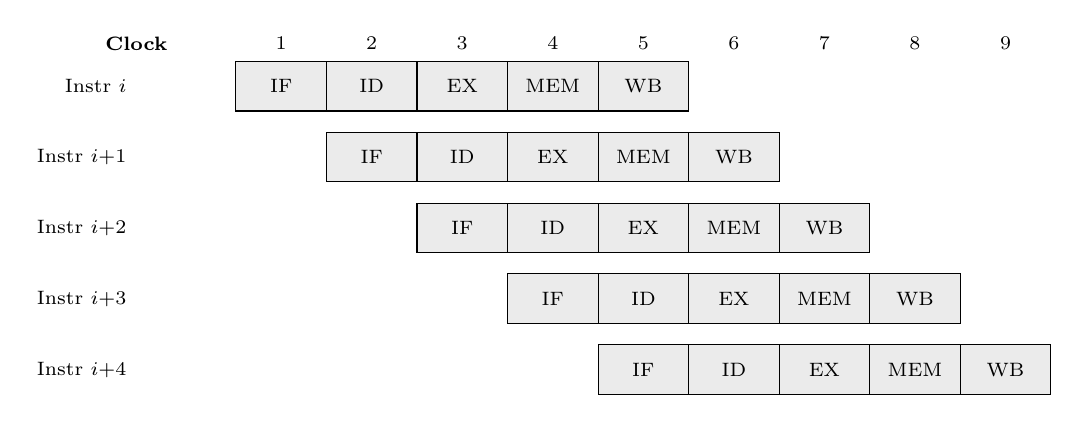
\begin{tikzpicture}[x=1.15cm,y=-0.9cm,font=\scriptsize]
  \foreach \x in {1,...,9} \node at (\x-0.5,-0.6) {\x};
  \node at (-1.1,-0.6) {\bfseries Clock};
  \foreach \i/\row/\name in {0/0/Instr $i$,1/1/Instr $i{+}1$,2/2/Instr $i{+}2$,3/3/Instr $i{+}3$,4/4/Instr $i{+}4$}{
    \node[left] at (-1.1,\row) {\name};
    \foreach \stage [count=\xi from 0] in {IF,ID,EX,MEM,WB}{
      \pgfmathsetmacro{\xoff}{\i+\xi}
      \draw[fill=black!8] (\xoff,\row-0.35) rectangle ++(1,0.7) node[midway]{\stage};
    }
  }
\end{tikzpicture}
\diagramsource{\nolinkurl{03-pipelining-lecture.pdf}, slide 25 (``MIPS In-Order Single-Issue Integer Pipeline Ideal Operation''); cf.\ H\&P Fig.~C.1, \hppage{C}{7}}
\end{minipage}
\end{center}

IF = Instruction Fetch, ID = Instruction Decode, EX = Execution,
MEM = Memory Access, WB = Write Back.
\emph{In-order} = instructions execute in original program order.
\emph{Ideal} = pipeline operation without any stall cycles.

\subsubsection{5 steps of the MIPS datapath (with pipeline registers)}

Data is carried from one stage to the next in \textbf{pipeline
registers/latches} (IF/ID, ID/EX, EX/MEM, MEM/WB), which hold temporary
values between clocks and the info needed for later stages.

\begin{center}\begin{minipage}{\linewidth}\centering
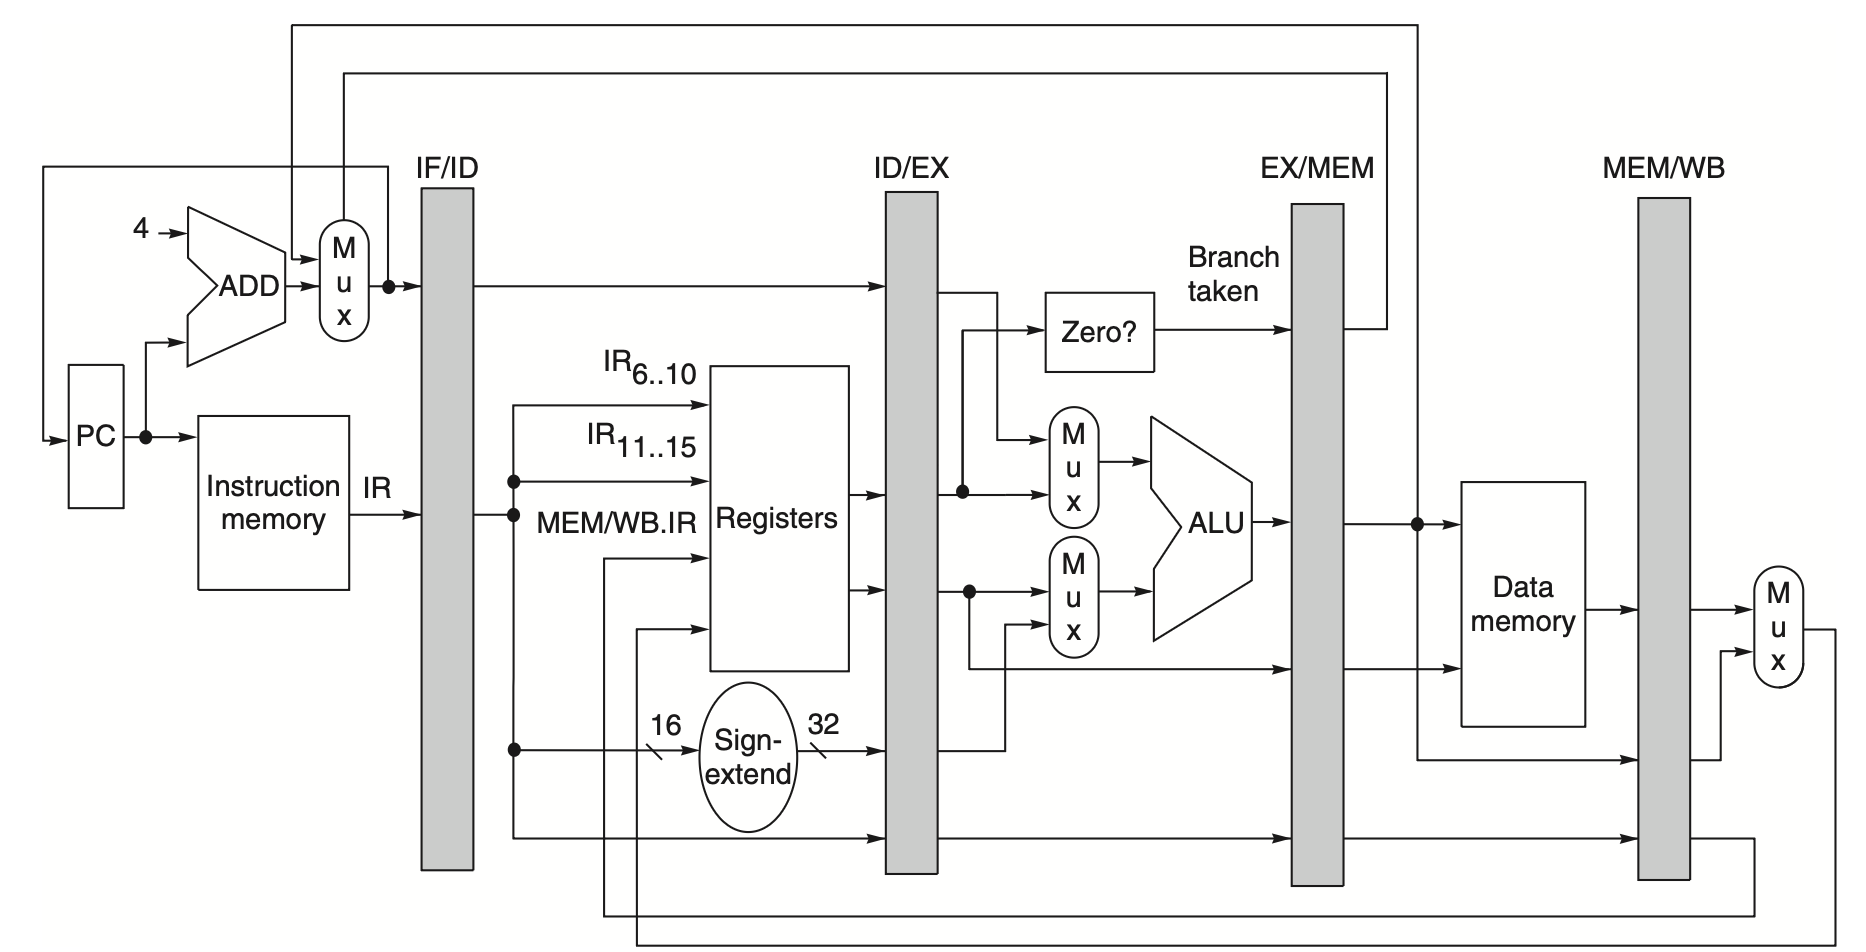
\includegraphics[width=\linewidth]{assets/figures/diag-36.png}
\diagramsource{H\&P Fig.~C.22, \hppage{C}{35} (image supplied by the note-taker); the same datapath as \nolinkurl{03-pipelining-lecture.pdf}, slide 26 (``5 Steps of MIPS Datapath'')}
\end{minipage}
\end{center}

Note: this is a \emph{data-stationary} control scheme -- each pipeline stage
locally decodes the control signals it needs from the instruction bits
carried along in the pipeline registers.

\subsubsection{Visualizing the pipeline (register read/write timing)}

\begin{center}\begin{minipage}{\linewidth}\centering
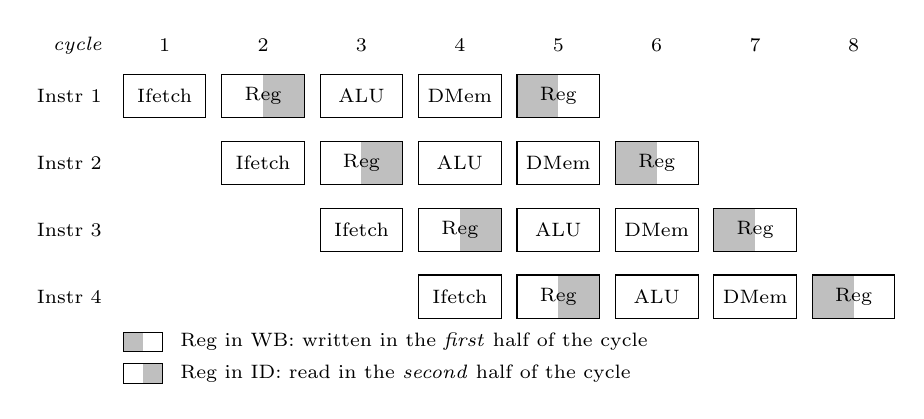
\begin{tikzpicture}[font=\scriptsize]
  \node[anchor=east,font=\scriptsize\itshape] at (-0.15,0.64) {cycle};
  \node at (0.525,0.64) {1};
  \node at (1.775,0.64) {2};
  \node at (3.025,0.64) {3};
  \node at (4.275,0.64) {4};
  \node at (5.525,0.64) {5};
  \node at (6.775,0.64) {6};
  \node at (8.025,0.64) {7};
  \node at (9.275,0.64) {8};
  \node[anchor=east] at (-0.15,0.000) {Instr 1};
  \draw (0.000,-0.275) rectangle (1.050,0.275);
  \node at (0.525,0.000) {Ifetch};
  \fill[black!25] (1.775,-0.275) rectangle (2.300,0.275);
  \draw (1.250,-0.275) rectangle (2.300,0.275);
  \node at (1.775,0.000) {Reg};
  \draw (2.500,-0.275) rectangle (3.550,0.275);
  \node at (3.025,0.000) {ALU};
  \draw (3.750,-0.275) rectangle (4.800,0.275);
  \node at (4.275,0.000) {DMem};
  \fill[black!25] (5.000,-0.275) rectangle (5.525,0.275);
  \draw (5.000,-0.275) rectangle (6.050,0.275);
  \node at (5.525,0.000) {Reg};
  \node[anchor=east] at (-0.15,-0.850) {Instr 2};
  \draw (1.250,-1.125) rectangle (2.300,-0.575);
  \node at (1.775,-0.850) {Ifetch};
  \fill[black!25] (3.025,-1.125) rectangle (3.550,-0.575);
  \draw (2.500,-1.125) rectangle (3.550,-0.575);
  \node at (3.025,-0.850) {Reg};
  \draw (3.750,-1.125) rectangle (4.800,-0.575);
  \node at (4.275,-0.850) {ALU};
  \draw (5.000,-1.125) rectangle (6.050,-0.575);
  \node at (5.525,-0.850) {DMem};
  \fill[black!25] (6.250,-1.125) rectangle (6.775,-0.575);
  \draw (6.250,-1.125) rectangle (7.300,-0.575);
  \node at (6.775,-0.850) {Reg};
  \node[anchor=east] at (-0.15,-1.700) {Instr 3};
  \draw (2.500,-1.975) rectangle (3.550,-1.425);
  \node at (3.025,-1.700) {Ifetch};
  \fill[black!25] (4.275,-1.975) rectangle (4.800,-1.425);
  \draw (3.750,-1.975) rectangle (4.800,-1.425);
  \node at (4.275,-1.700) {Reg};
  \draw (5.000,-1.975) rectangle (6.050,-1.425);
  \node at (5.525,-1.700) {ALU};
  \draw (6.250,-1.975) rectangle (7.300,-1.425);
  \node at (6.775,-1.700) {DMem};
  \fill[black!25] (7.500,-1.975) rectangle (8.025,-1.425);
  \draw (7.500,-1.975) rectangle (8.550,-1.425);
  \node at (8.025,-1.700) {Reg};
  \node[anchor=east] at (-0.15,-2.550) {Instr 4};
  \draw (3.750,-2.825) rectangle (4.800,-2.275);
  \node at (4.275,-2.550) {Ifetch};
  \fill[black!25] (5.525,-2.825) rectangle (6.050,-2.275);
  \draw (5.000,-2.825) rectangle (6.050,-2.275);
  \node at (5.525,-2.550) {Reg};
  \draw (6.250,-2.825) rectangle (7.300,-2.275);
  \node at (6.775,-2.550) {ALU};
  \draw (7.500,-2.825) rectangle (8.550,-2.275);
  \node at (8.025,-2.550) {DMem};
  \fill[black!25] (8.750,-2.825) rectangle (9.275,-2.275);
  \draw (8.750,-2.825) rectangle (9.800,-2.275);
  \node at (9.275,-2.550) {Reg};
  \fill[black!25] (0,-3.25) rectangle ++(0.25,0.25); \draw (0,-3.25) rectangle ++(0.5,0.25);
  \node[anchor=west] at (0.6,-3.125) {Reg in WB: written in the \emph{first} half of the cycle};
  \fill[black!25] (0.25,-3.65) rectangle ++(0.25,0.25); \draw (0,-3.65) rectangle ++(0.5,0.25);
  \node[anchor=west] at (0.6,-3.525) {Reg in ID: read in the \emph{second} half of the cycle};
\end{tikzpicture}
\diagramsource{\nolinkurl{03-pipelining-lecture.pdf}, slide 27 (``Visualizing Pipelining''); cf.\ H\&P Fig.~C.3, \hppage{C}{9}}
\end{minipage}
\end{center}

\begin{itemize}
  \item Read operand registers in the \textbf{second half} of the ID cycle.
  \item Write the destination register in the \textbf{first half} of the WB
  cycle.
\end{itemize}
This is an ideal integer in-order 5-stage pipeline.

\subsubsection{Pipelining performance example}

\begin{eg}[Pipelining a multi-cycle CPU]
For an unpipelined CPU: clock cycle $=1$ns; 4 cycles for ALU
operations/branches, 5 cycles for memory operations; instruction mix
$40\%/20\%/40\%$ (ALU/branch/memory). Pipelining adds 0.2ns to the clock
cycle.

\[
  \text{Non-pipelined avg.\ instr.\ time} = 1\text{ns}\times((40\%+20\%)\times4 + 40\%\times5) = 4.4\text{ns}
\]
\[
  \text{Pipelined avg.\ instr.\ time} = 1\text{ns} + 0.2\text{ns} = 1.2\text{ns}
\]
\[
  \text{Speedup} = \frac{4.4}{1.2} = 3.7 \times \text{ faster}
\]
\end{eg}

\subsection{Pipeline Hazards}
\label{sec:hazards}

\subsubsection{Three Kinds of Hazards}
\label{sec:hazard-types}

\begin{definition}[Pipeline hazards]
\textbf{Hazards} are situations in pipelining that prevent the next
instruction in the instruction stream from executing during its designated
clock cycle, possibly resulting in one or more \emph{stall} (wait) cycles.
Hazards increase CPI above 1 and are classified into three types:

\begin{itemize}
  \item \textbf{Structural hazards}: arise from hardware resource conflicts
  when available hardware cannot support all possible combinations of
  instructions.
  \item \textbf{Data hazards}: arise when an instruction depends on the
  result of a previous instruction in a way exposed by the overlapping of
  instructions in the pipeline.
  \item \textbf{Control hazards}: arise from the pipelining of conditional
  branches and other instructions that change the PC.
\end{itemize}\HPA{C}{\S C.2}{11}
\end{definition}

\begin{note}
An instruction ``issued later'' than instruction $x$
was issued after $x$ and is \emph{not as far along} in the pipeline. An
instruction ``issued earlier'' than $x$ was issued before $x$ and is
\emph{further along} in the pipeline.
\end{note}

\paragraph{Stalls and performance}

Stalls impede progress of a pipeline and cause deviation from 1
instruction/cycle.
\begin{prop}[CPI and speedup with stalls]
\[
  \mathrm{CPI}_{\text{pipelined}} = \text{Ideal CPI} + \text{Pipeline stall cycles per instruction} = 1 + \text{stall cycles/instr.}
\]
Ignoring overhead, assuming balanced stages:
\[
  \text{Speedup} = \frac{\mathrm{CPI}_{\text{unpipelined}}}{1 + \text{pipeline stall cycles per instruction}}
\]\HPA[13]{C}{\S C.2}{12}
\end{prop}

\subsubsection{Structural Hazards}
\label{sec:structural-hazards}

\begin{definition}[Structural hazard]
In pipelined machines, overlapped instruction execution requires pipelining
of functional units and duplication of resources so all possible
instruction combinations can be supported. If a \textbf{resource conflict}
arises because a hardware resource is required by more than one instruction
in a single cycle, and it cannot be accommodated, a \textbf{structural
hazard} occurs -- e.g.\ a pipelined machine with a single shared memory port
for instructions and data $\Rightarrow$ stall the pipeline for one cycle for
a memory data access.\HPA[15]{C}{\S C.2}{13}
\end{definition}

\paragraph{Example: single shared memory port}

\begin{center}\begin{minipage}{\linewidth}\centering
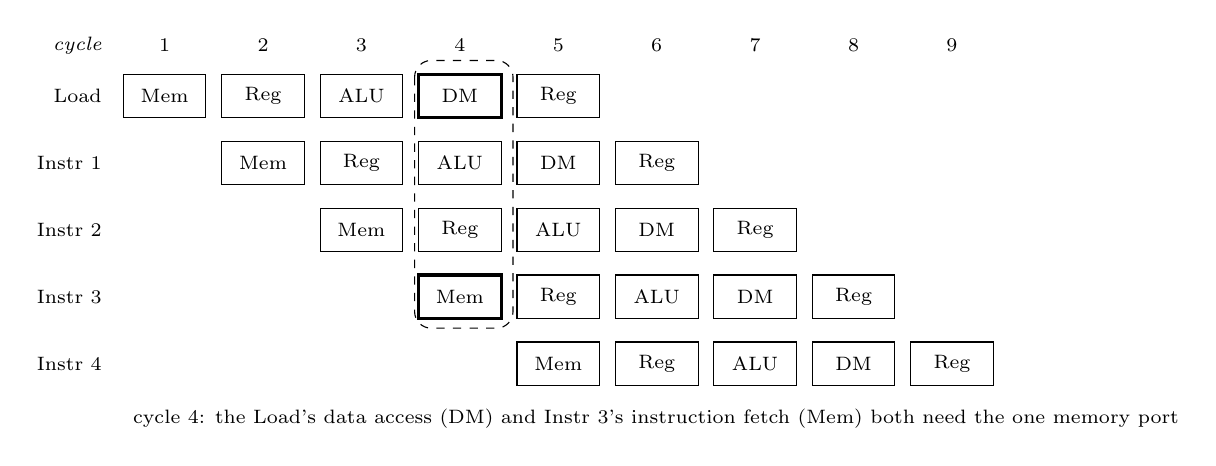
\begin{tikzpicture}[font=\scriptsize]
  \node[anchor=east,font=\scriptsize\itshape] at (-0.15,0.64) {cycle};
  \node at (0.525,0.64) {1};
  \node at (1.775,0.64) {2};
  \node at (3.025,0.64) {3};
  \node at (4.275,0.64) {4};
  \node at (5.525,0.64) {5};
  \node at (6.775,0.64) {6};
  \node at (8.025,0.64) {7};
  \node at (9.275,0.64) {8};
  \node at (10.525,0.64) {9};
  \node[anchor=east] at (-0.15,0.000) {Load};
  \draw (0.000,-0.275) rectangle (1.050,0.275);
  \node at (0.525,0.000) {Mem};
  \draw (1.250,-0.275) rectangle (2.300,0.275);
  \node at (1.775,0.000) {Reg};
  \draw (2.500,-0.275) rectangle (3.550,0.275);
  \node at (3.025,0.000) {ALU};
  \draw[very thick] (3.750,-0.275) rectangle (4.800,0.275);
  \node at (4.275,0.000) {DM};
  \draw (5.000,-0.275) rectangle (6.050,0.275);
  \node at (5.525,0.000) {Reg};
  \node[anchor=east] at (-0.15,-0.850) {Instr 1};
  \draw (1.250,-1.125) rectangle (2.300,-0.575);
  \node at (1.775,-0.850) {Mem};
  \draw (2.500,-1.125) rectangle (3.550,-0.575);
  \node at (3.025,-0.850) {Reg};
  \draw (3.750,-1.125) rectangle (4.800,-0.575);
  \node at (4.275,-0.850) {ALU};
  \draw (5.000,-1.125) rectangle (6.050,-0.575);
  \node at (5.525,-0.850) {DM};
  \draw (6.250,-1.125) rectangle (7.300,-0.575);
  \node at (6.775,-0.850) {Reg};
  \node[anchor=east] at (-0.15,-1.700) {Instr 2};
  \draw (2.500,-1.975) rectangle (3.550,-1.425);
  \node at (3.025,-1.700) {Mem};
  \draw (3.750,-1.975) rectangle (4.800,-1.425);
  \node at (4.275,-1.700) {Reg};
  \draw (5.000,-1.975) rectangle (6.050,-1.425);
  \node at (5.525,-1.700) {ALU};
  \draw (6.250,-1.975) rectangle (7.300,-1.425);
  \node at (6.775,-1.700) {DM};
  \draw (7.500,-1.975) rectangle (8.550,-1.425);
  \node at (8.025,-1.700) {Reg};
  \node[anchor=east] at (-0.15,-2.550) {Instr 3};
  \draw[very thick] (3.750,-2.825) rectangle (4.800,-2.275);
  \node at (4.275,-2.550) {Mem};
  \draw (5.000,-2.825) rectangle (6.050,-2.275);
  \node at (5.525,-2.550) {Reg};
  \draw (6.250,-2.825) rectangle (7.300,-2.275);
  \node at (6.775,-2.550) {ALU};
  \draw (7.500,-2.825) rectangle (8.550,-2.275);
  \node at (8.025,-2.550) {DM};
  \draw (8.750,-2.825) rectangle (9.800,-2.275);
  \node at (9.275,-2.550) {Reg};
  \node[anchor=east] at (-0.15,-3.400) {Instr 4};
  \draw (5.000,-3.675) rectangle (6.050,-3.125);
  \node at (5.525,-3.400) {Mem};
  \draw (6.250,-3.675) rectangle (7.300,-3.125);
  \node at (6.775,-3.400) {Reg};
  \draw (7.500,-3.675) rectangle (8.550,-3.125);
  \node at (8.025,-3.400) {ALU};
  \draw (8.750,-3.675) rectangle (9.800,-3.125);
  \node at (9.275,-3.400) {DM};
  \draw (10.000,-3.675) rectangle (11.050,-3.125);
  \node at (10.525,-3.400) {Reg};
  \draw[dashed,rounded corners=6pt] (3.70,0.45) rectangle (4.95,-2.95);
  \node[anchor=north west,font=\scriptsize] at (0,-3.85) {cycle 4: the Load's data access (DM) and Instr 3's instruction fetch (Mem) both need the one memory port};
\end{tikzpicture}
\diagramsource{\nolinkurl{03-pipelining-lecture.pdf}, slide 33 (``An example of a structural hazard''); cf.\ H\&P Fig.~C.4, \hppage{C}{14}}
\end{minipage}
\end{center}

\textbf{Resolution: stall (insert a bubble/NOP).}

\begin{center}\begin{minipage}{\linewidth}\centering
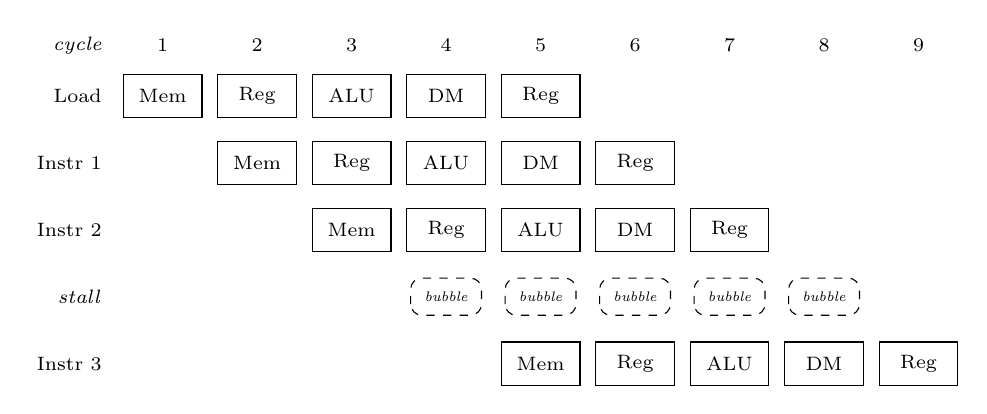
\begin{tikzpicture}[font=\scriptsize]
  \node[anchor=east,font=\scriptsize\itshape] at (-0.15,0.64) {cycle};
  \node at (0.500,0.64) {1};
  \node at (1.700,0.64) {2};
  \node at (2.900,0.64) {3};
  \node at (4.100,0.64) {4};
  \node at (5.300,0.64) {5};
  \node at (6.500,0.64) {6};
  \node at (7.700,0.64) {7};
  \node at (8.900,0.64) {8};
  \node at (10.100,0.64) {9};
  \node[anchor=east] at (-0.15,0.000) {Load};
  \draw (0.000,-0.275) rectangle (1.000,0.275);
  \node at (0.500,0.000) {Mem};
  \draw (1.200,-0.275) rectangle (2.200,0.275);
  \node at (1.700,0.000) {Reg};
  \draw (2.400,-0.275) rectangle (3.400,0.275);
  \node at (2.900,0.000) {ALU};
  \draw (3.600,-0.275) rectangle (4.600,0.275);
  \node at (4.100,0.000) {DM};
  \draw (4.800,-0.275) rectangle (5.800,0.275);
  \node at (5.300,0.000) {Reg};
  \node[anchor=east] at (-0.15,-0.850) {Instr 1};
  \draw (1.200,-1.125) rectangle (2.200,-0.575);
  \node at (1.700,-0.850) {Mem};
  \draw (2.400,-1.125) rectangle (3.400,-0.575);
  \node at (2.900,-0.850) {Reg};
  \draw (3.600,-1.125) rectangle (4.600,-0.575);
  \node at (4.100,-0.850) {ALU};
  \draw (4.800,-1.125) rectangle (5.800,-0.575);
  \node at (5.300,-0.850) {DM};
  \draw (6.000,-1.125) rectangle (7.000,-0.575);
  \node at (6.500,-0.850) {Reg};
  \node[anchor=east] at (-0.15,-1.700) {Instr 2};
  \draw (2.400,-1.975) rectangle (3.400,-1.425);
  \node at (2.900,-1.700) {Mem};
  \draw (3.600,-1.975) rectangle (4.600,-1.425);
  \node at (4.100,-1.700) {Reg};
  \draw (4.800,-1.975) rectangle (5.800,-1.425);
  \node at (5.300,-1.700) {ALU};
  \draw (6.000,-1.975) rectangle (7.000,-1.425);
  \node at (6.500,-1.700) {DM};
  \draw (7.200,-1.975) rectangle (8.200,-1.425);
  \node at (7.700,-1.700) {Reg};
  \node[anchor=east] at (-0.15,-2.550) {\emph{stall}};
  \draw[dashed,rounded corners=4pt] (3.650,-2.785) rectangle (4.550,-2.315);
  \node[font=\tiny\itshape] at (4.100,-2.550) {bubble};
  \draw[dashed,rounded corners=4pt] (4.850,-2.785) rectangle (5.750,-2.315);
  \node[font=\tiny\itshape] at (5.300,-2.550) {bubble};
  \draw[dashed,rounded corners=4pt] (6.050,-2.785) rectangle (6.950,-2.315);
  \node[font=\tiny\itshape] at (6.500,-2.550) {bubble};
  \draw[dashed,rounded corners=4pt] (7.250,-2.785) rectangle (8.150,-2.315);
  \node[font=\tiny\itshape] at (7.700,-2.550) {bubble};
  \draw[dashed,rounded corners=4pt] (8.450,-2.785) rectangle (9.350,-2.315);
  \node[font=\tiny\itshape] at (8.900,-2.550) {bubble};
  \node[anchor=east] at (-0.15,-3.400) {Instr 3};
  \draw (4.800,-3.675) rectangle (5.800,-3.125);
  \node at (5.300,-3.400) {Mem};
  \draw (6.000,-3.675) rectangle (7.000,-3.125);
  \node at (6.500,-3.400) {Reg};
  \draw (7.200,-3.675) rectangle (8.200,-3.125);
  \node at (7.700,-3.400) {ALU};
  \draw (8.400,-3.675) rectangle (9.400,-3.125);
  \node at (8.900,-3.400) {DM};
  \draw (9.600,-3.675) rectangle (10.600,-3.125);
  \node at (10.100,-3.400) {Reg};

\end{tikzpicture}
\diagramsource{\nolinkurl{03-pipelining-lecture.pdf}, slide 34 (``How is it resolved?''); cf.\ H\&P Fig.~C.5, \hppage{C}{15}}
\end{minipage}
\end{center}

\paragraph{Structural hazard: numeric example}

\begin{eg}[Is a structural hazard worth it?]
Given data references are $40\%$ of a program, ideal pipelined CPI $=1$. A
machine with a data-memory structural hazard needs 1 stall cycle per data
reference, but its clock rate is $1.05\times$ higher than the ideal
machine:
\[
  \text{Avg.\ instr.\ time} = (1+0.4\times1)\times\frac{\text{Clock}_{\text{ideal}}}{1.05} = 1.3\times \text{Clock}_{\text{ideal}}
\]
$\Rightarrow$ the machine \emph{without} the hazard is still better ($1.3 >
1$).
\end{eg}

\begin{remark}
\textbf{Remember the common case!} All else equal, a machine without
structural hazards always has lower CPI, but sometimes it is cheaper (in
hardware) to allow a hazard than to eliminate it -- weigh HW cost of
pipelining/duplicating a unit against how often the hazard actually occurs.
\end{remark}

\subsubsection{Data Hazards}
\label{sec:data-hazards}

\begin{definition}[Data hazard]
Data hazards occur when the pipeline changes the order of read/write
accesses to operands compared to the original sequential order, potentially
causing \textbf{incorrect execution}. One or more instructions may need to
stall to ensure correctness.\HPA{C}{\S C.2}{15}
\end{definition}

\begin{eg}[RAW on R1]
\leavevmode
\begin{lstlisting}
ADD R1, R2, R3
SUB R4, R1, R5
AND R6, R1, R7
OR  R8, R1, R9
XOR R10, R1, R11
\end{lstlisting}
All instructions after \texttt{ADD} use its result (\texttt{R1}); \texttt{SUB}
and \texttt{AND} would need to stall for correct execution without
forwarding.
\end{eg}

\paragraph{Data Hazard Classification}

\begin{definition}[RAW, WAW, WAR]
Given two instructions $I$, $J$, with $I$ occurring before $J$ in program
order:

\begin{itemize}
  \item \textbf{RAW} (read after write) -- \emph{true data dependence}: $J$
  tries to read a source before $I$ writes it, so $J$ incorrectly gets the
  old value.
  \item \textbf{WAW} (write after write) -- \emph{name dependence}: $J$
  tries to write an operand before it is written by $I$; the writes end up
  performed in the wrong order.
  \item \textbf{WAR} (write after read) -- \emph{name dependence}: $J$
  tries to write a destination before it is read by $I$, so $I$ incorrectly
  gets the new value.
  \item \textbf{RAR} (read after read): \emph{not} a hazard.
\end{itemize}\HP{\S3.1, Data Hazards}{153}
\end{definition}

\begin{center}\begin{minipage}{\linewidth}\centering
\begin{tikzpicture}[font=\small]
  \draw[-{Latex}] (-1.6,1.3) -- (-1.6,0) node[midway,left,font=\scriptsize,align=right] {program\\order};
  \begin{scope}[xshift=0.00cm]
  \node[draw,minimum width=1.9cm] (I) at (0,1.3) {$I$ (Write)};
  \node[draw,minimum width=1.9cm] (J) at (0,0) {$J$ (Read)};
  \node[draw,align=center] (S) at (2.7,0.65) {Shared\\operand};
  \draw[-{Latex}] (I.east) -- (S.north west);
  \draw[-{Latex}] (S.south west) -- (J.east);
  \node[font=\small\bfseries,align=center] at (1.35,-0.75) {RAW (true dependence)};
  \end{scope}
  \begin{scope}[xshift=6.20cm]
  \node[draw,minimum width=1.9cm] (I) at (0,1.3) {$I$ (Read)};
  \node[draw,minimum width=1.9cm] (J) at (0,0) {$J$ (Write)};
  \node[draw,align=center] (S) at (2.7,0.65) {Shared\\operand};
  \draw[-{Latex}] (S.north west) -- (I.east);
  \draw[-{Latex}] (J.east) -- (S.south west);
  \node[font=\small\bfseries,align=center] at (1.35,-0.75) {WAR (name dependence)};
  \end{scope}
\end{tikzpicture}
\diagramsource{\nolinkurl{03-pipelining-lecture.pdf}, slide 45 (``Data Hazard Classification'') (RAW, WAR)}
\end{minipage}
\end{center}

\begin{center}\begin{minipage}{\linewidth}\centering
\begin{tikzpicture}[font=\small]
  \draw[-{Latex}] (-1.6,1.3) -- (-1.6,0) node[midway,left,font=\scriptsize,align=right] {program\\order};
  \begin{scope}[xshift=0.00cm]
  \node[draw,minimum width=1.9cm] (I) at (0,1.3) {$I$ (Write)};
  \node[draw,minimum width=1.9cm] (J) at (0,0) {$J$ (Write)};
  \node[draw,align=center] (S) at (2.7,0.65) {Shared\\operand};
  \draw[-{Latex}] (I.east) -- (S.north west);
  \draw[-{Latex}] (J.east) -- (S.south west);
  \node[font=\small\bfseries,align=center] at (1.35,-0.75) {WAW (name dependence)};
  \end{scope}
  \begin{scope}[xshift=6.20cm]
  \node[draw,minimum width=1.9cm] (I) at (0,1.3) {$I$ (Read)};
  \node[draw,minimum width=1.9cm] (J) at (0,0) {$J$ (Read)};
  \node[draw,align=center] (S) at (2.7,0.65) {Shared\\operand};
  \draw[-{Latex}] (S.north west) -- (I.east);
  \draw[-{Latex}] (S.south west) -- (J.east);
  \node[font=\small\bfseries,align=center] at (1.35,-0.75) {RAR (\emph{not} a hazard)};
  \end{scope}
\end{tikzpicture}
\diagramsource{\nolinkurl{03-pipelining-lecture.pdf}, slide 45 (``Data Hazard Classification'') (WAW, RAR)}
\end{minipage}
\end{center}

\begin{itemize}
  \item \textbf{RAW example:} \texttt{i: ADD R1,R2,R3} \quad
        \texttt{j: SUB R4,R1,R6}
  \item \textbf{WAW example:} \texttt{i: SUB R1,R4,R3} \quad
        \texttt{j: ADD R1,R2,R3}
  \item \textbf{WAR example:} \texttt{i: SUB R4,R1,R3} \quad
        \texttt{j: ADD R1,R2,R3}
\end{itemize}
\begin{remark}
RAW and WAW can be resolved with stalling or forwarding; WAR does not occur
in the simple MIPS pipeline because reads happen early (ID) and writes late
(WB) in program order, so instructions never write before an earlier one has
read (only relevant for pipelines that reorder execution).
\end{remark}

\paragraph{Data hazard on R1 (visualized)}

\begin{center}\begin{minipage}{\linewidth}\centering
\begin{tikzpicture}[font=\scriptsize]
  \node[anchor=east,font=\scriptsize\itshape] at (-0.15,0.64) {cycle};
  \node at (0.525,0.64) {1};
  \node at (1.775,0.64) {2};
  \node at (3.025,0.64) {3};
  \node at (4.275,0.64) {4};
  \node at (5.525,0.64) {5};
  \node at (6.775,0.64) {6};
  \node at (8.025,0.64) {7};
  \node at (9.275,0.64) {8};
  \node at (10.525,0.64) {9};
  \node[anchor=east] at (-0.15,0.000) {\texttt{add r1,r2,r3}};
  \draw (0.000,-0.275) rectangle (1.050,0.275);
  \node at (0.525,0.000) {Ifetch};
  \draw (1.250,-0.275) rectangle (2.300,0.275);
  \node at (1.775,0.000) {Reg};
  \draw (2.500,-0.275) rectangle (3.550,0.275);
  \node at (3.025,0.000) {ALU};
  \draw (3.750,-0.275) rectangle (4.800,0.275);
  \node at (4.275,0.000) {DMem};
  \draw (5.000,-0.275) rectangle (6.050,0.275);
  \node at (5.525,0.000) {Reg};
  \node[anchor=east] at (-0.15,-0.850) {\texttt{sub r4,r1,r3}};
  \draw (1.250,-1.125) rectangle (2.300,-0.575);
  \node at (1.775,-0.850) {Ifetch};
  \draw (2.500,-1.125) rectangle (3.550,-0.575);
  \node at (3.025,-0.850) {Reg};
  \draw (3.750,-1.125) rectangle (4.800,-0.575);
  \node at (4.275,-0.850) {ALU};
  \draw (5.000,-1.125) rectangle (6.050,-0.575);
  \node at (5.525,-0.850) {DMem};
  \draw (6.250,-1.125) rectangle (7.300,-0.575);
  \node at (6.775,-0.850) {Reg};
  \node[anchor=east] at (-0.15,-1.700) {\texttt{and r6,r1,r7}};
  \draw (2.500,-1.975) rectangle (3.550,-1.425);
  \node at (3.025,-1.700) {Ifetch};
  \draw (3.750,-1.975) rectangle (4.800,-1.425);
  \node at (4.275,-1.700) {Reg};
  \draw (5.000,-1.975) rectangle (6.050,-1.425);
  \node at (5.525,-1.700) {ALU};
  \draw (6.250,-1.975) rectangle (7.300,-1.425);
  \node at (6.775,-1.700) {DMem};
  \draw (7.500,-1.975) rectangle (8.550,-1.425);
  \node at (8.025,-1.700) {Reg};
  \node[anchor=east] at (-0.15,-2.550) {\texttt{or\ \ r8,r1,r9}};
  \draw (3.750,-2.825) rectangle (4.800,-2.275);
  \node at (4.275,-2.550) {Ifetch};
  \draw (5.000,-2.825) rectangle (6.050,-2.275);
  \node at (5.525,-2.550) {Reg};
  \draw (6.250,-2.825) rectangle (7.300,-2.275);
  \node at (6.775,-2.550) {ALU};
  \draw (7.500,-2.825) rectangle (8.550,-2.275);
  \node at (8.025,-2.550) {DMem};
  \draw (8.750,-2.825) rectangle (9.800,-2.275);
  \node at (9.275,-2.550) {Reg};
  \node[anchor=east] at (-0.15,-3.400) {\texttt{xor r10,r1,r11}};
  \draw (5.000,-3.675) rectangle (6.050,-3.125);
  \node at (5.525,-3.400) {Ifetch};
  \draw (6.250,-3.675) rectangle (7.300,-3.125);
  \node at (6.775,-3.400) {Reg};
  \draw (7.500,-3.675) rectangle (8.550,-3.125);
  \node at (8.025,-3.400) {ALU};
  \draw (8.750,-3.675) rectangle (9.800,-3.125);
  \node at (9.275,-3.400) {DMem};
  \draw (10.000,-3.675) rectangle (11.050,-3.125);
  \node at (10.525,-3.400) {Reg};
  \draw[-{Latex[length=2mm]},thick,solid] (4.900,-0.275) -- (3.025,-0.575);
  \draw[-{Latex[length=2mm]},thick,solid] (4.900,-0.275) -- (4.900,-1.275) -- (4.275,-1.425);
  \draw[-{Latex[length=2mm]},thick,dashed] (6.150,-0.275) -- (6.150,-2.125) -- (5.525,-2.275);
  \draw[-{Latex[length=2mm]},thick,dashed] (6.150,-0.275) -- (6.150,-2.975) -- (6.775,-3.125);
  \draw[thick,-{Latex[length=2mm]}] (0,-4.1) -- (0.7,-4.1); \node[anchor=west] at (0.8,-4.1) {needed before \texttt{add} writes \texttt{r1}: hazard};
  \draw[thick,dashed,-{Latex[length=2mm]}] (0,-4.5) -- (0.7,-4.5); \node[anchor=west] at (0.8,-4.5) {read after the write (WB first half): no hazard};
\end{tikzpicture}
\diagramsource{\nolinkurl{03-pipelining-lecture.pdf}, slide 39 (``Data Hazard on R1''); cf.\ H\&P Fig.~C.6, \hppage{C}{17}}
\end{minipage}
\end{center}
Without forwarding, \texttt{add}'s result is only available (written back)
after its WB stage, but \texttt{sub} needs \texttt{r1} in its ID stage one
cycle earlier -- a RAW hazard.

\subsubsection{Minimizing Data Hazard Stalls by Forwarding}
\label{sec:forwarding}

\begin{definition}[Forwarding]
\textbf{Forwarding} (a.k.a.\ \emph{register bypassing} or
\emph{short-circuiting}) is a hardware-based technique used to eliminate or
minimize data-hazard stalls. The result of an instruction is copied directly
from where it is produced (ALU output, memory read port, etc.) to where a
subsequent instruction needs it (ALU input register, memory write port,
etc.), \emph{without} waiting for it to be written to and re-read from the
register file.\HPA[18]{C}{\S C.2}{16}
\end{definition}

In the MIPS integer pipeline with forwarding:
\begin{itemize}
  \item The \textbf{ALU result} from the EX/MEM register may be forwarded
  back to the ALU input latches instead of the register value read in ID.
  \item The \textbf{Data Memory result} from the MEM/WB register may also be
  forwarded to the ALU input latches.
  \item If the forwarding hardware detects that a previous ALU operation
  will write the register that is a source for the current ALU operation,
  control logic selects the forwarded result as the ALU input instead of the
  value read from the register file.
\end{itemize}

\paragraph{Datapath modified for forwarding}

\begin{center}\begin{minipage}{\linewidth}\centering
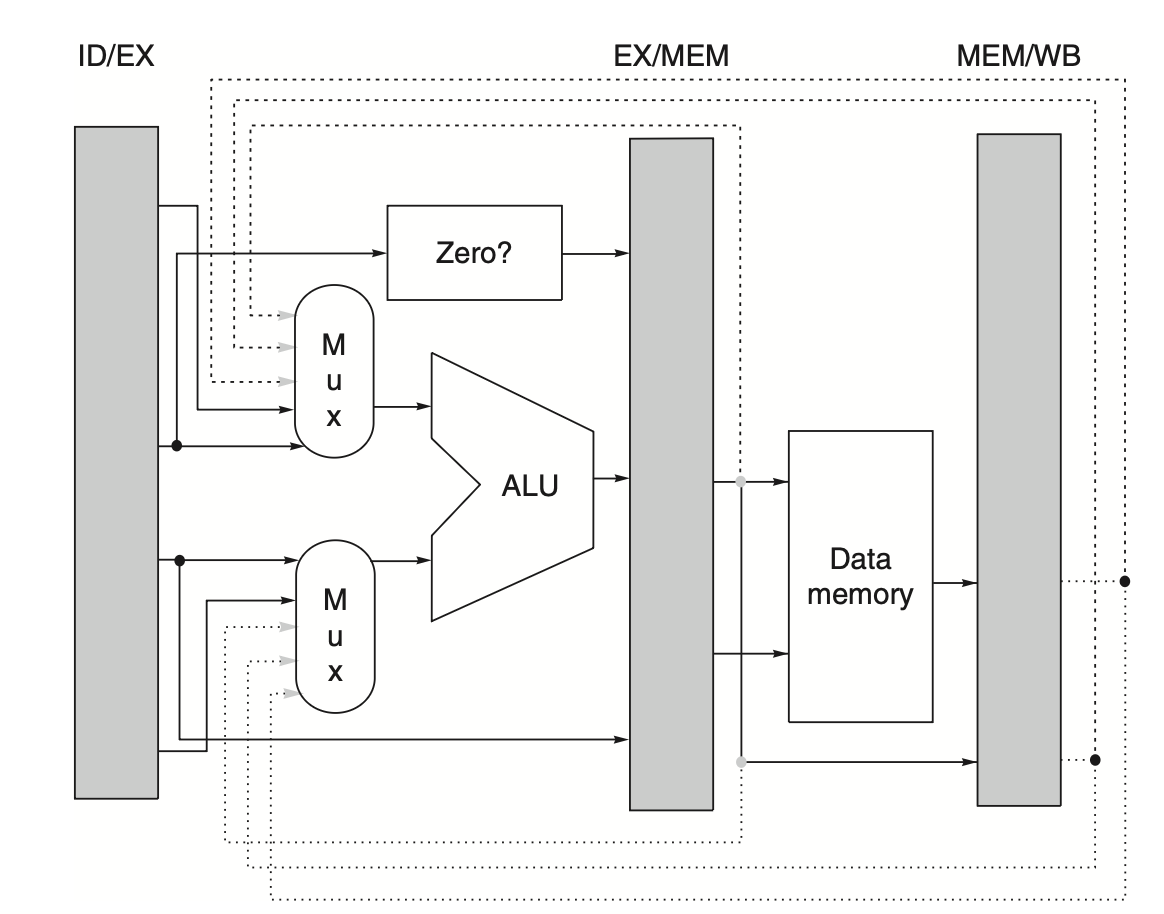
\includegraphics[width=0.7\linewidth]{assets/figures/diag-43.png}
\diagramsource{H\&P Fig.~C.27, \hppage{C}{41} (image supplied by the note-taker; dotted lines are the forwarding paths); cf.\ \nolinkurl{03-pipelining-lecture.pdf}, slide 41 (``HW Change for Forwarding'')}
\end{minipage}
\end{center}
Red paths show the EX/MEM $\to$ ALU-input and MEM/WB $\to$ ALU-input
forwarding routes, plus the normal write-back path to the register file.

\paragraph{Forwarding to avoid the RAW hazard}

\begin{center}\begin{minipage}{\linewidth}\centering
\begin{tikzpicture}[font=\scriptsize]
  \node[anchor=east,font=\scriptsize\itshape] at (-0.15,0.64) {cycle};
  \node at (0.525,0.64) {1};
  \node at (1.775,0.64) {2};
  \node at (3.025,0.64) {3};
  \node at (4.275,0.64) {4};
  \node at (5.525,0.64) {5};
  \node at (6.775,0.64) {6};
  \node at (8.025,0.64) {7};
  \node at (9.275,0.64) {8};
  \node at (10.525,0.64) {9};
  \node[anchor=east] at (-0.15,0.000) {\texttt{add r1,r2,r3}};
  \draw (0.000,-0.275) rectangle (1.050,0.275);
  \node at (0.525,0.000) {Ifetch};
  \draw (1.250,-0.275) rectangle (2.300,0.275);
  \node at (1.775,0.000) {Reg};
  \draw (2.500,-0.275) rectangle (3.550,0.275);
  \node at (3.025,0.000) {ALU};
  \draw (3.750,-0.275) rectangle (4.800,0.275);
  \node at (4.275,0.000) {DMem};
  \draw (5.000,-0.275) rectangle (6.050,0.275);
  \node at (5.525,0.000) {Reg};
  \node[anchor=east] at (-0.15,-0.850) {\texttt{sub r4,r1,r3}};
  \draw (1.250,-1.125) rectangle (2.300,-0.575);
  \node at (1.775,-0.850) {Ifetch};
  \draw (2.500,-1.125) rectangle (3.550,-0.575);
  \node at (3.025,-0.850) {Reg};
  \draw (3.750,-1.125) rectangle (4.800,-0.575);
  \node at (4.275,-0.850) {ALU};
  \draw (5.000,-1.125) rectangle (6.050,-0.575);
  \node at (5.525,-0.850) {DMem};
  \draw (6.250,-1.125) rectangle (7.300,-0.575);
  \node at (6.775,-0.850) {Reg};
  \node[anchor=east] at (-0.15,-1.700) {\texttt{and r6,r1,r7}};
  \draw (2.500,-1.975) rectangle (3.550,-1.425);
  \node at (3.025,-1.700) {Ifetch};
  \draw (3.750,-1.975) rectangle (4.800,-1.425);
  \node at (4.275,-1.700) {Reg};
  \draw (5.000,-1.975) rectangle (6.050,-1.425);
  \node at (5.525,-1.700) {ALU};
  \draw (6.250,-1.975) rectangle (7.300,-1.425);
  \node at (6.775,-1.700) {DMem};
  \draw (7.500,-1.975) rectangle (8.550,-1.425);
  \node at (8.025,-1.700) {Reg};
  \node[anchor=east] at (-0.15,-2.550) {\texttt{or\ \ r8,r1,r9}};
  \draw (3.750,-2.825) rectangle (4.800,-2.275);
  \node at (4.275,-2.550) {Ifetch};
  \draw (5.000,-2.825) rectangle (6.050,-2.275);
  \node at (5.525,-2.550) {Reg};
  \draw (6.250,-2.825) rectangle (7.300,-2.275);
  \node at (6.775,-2.550) {ALU};
  \draw (7.500,-2.825) rectangle (8.550,-2.275);
  \node at (8.025,-2.550) {DMem};
  \draw (8.750,-2.825) rectangle (9.800,-2.275);
  \node at (9.275,-2.550) {Reg};
  \node[anchor=east] at (-0.15,-3.400) {\texttt{xor r10,r1,r11}};
  \draw (5.000,-3.675) rectangle (6.050,-3.125);
  \node at (5.525,-3.400) {Ifetch};
  \draw (6.250,-3.675) rectangle (7.300,-3.125);
  \node at (6.775,-3.400) {Reg};
  \draw (7.500,-3.675) rectangle (8.550,-3.125);
  \node at (8.025,-3.400) {ALU};
  \draw (8.750,-3.675) rectangle (9.800,-3.125);
  \node at (9.275,-3.400) {DMem};
  \draw (10.000,-3.675) rectangle (11.050,-3.125);
  \node at (10.525,-3.400) {Reg};
  \draw[-{Latex[length=2mm]},thick,solid] (3.650,-0.275) -- (4.275,-0.575);
  \draw[-{Latex[length=2mm]},thick,solid] (4.900,-0.275) -- (4.900,-1.275) -- (5.525,-1.425);
  \draw[-{Latex[length=2mm]},thick,dashed] (6.150,-0.275) -- (6.150,-2.125) -- (5.525,-2.275);
  \draw[thick,-{Latex[length=2mm]}] (0,-4.1) -- (0.7,-4.1); \node[anchor=west] at (0.8,-4.1) {forwarded from EX/MEM or MEM/WB to the ALU};
  \draw[thick,dashed,-{Latex[length=2mm]}] (0,-4.5) -- (0.7,-4.5); \node[anchor=west] at (0.8,-4.5) {through the register file (write, then read)};
\end{tikzpicture}
\diagramsource{\nolinkurl{03-pipelining-lecture.pdf}, slide 42 (``Forwarding to Avoid Data Hazard''); cf.\ H\&P Fig.~C.7, \hppage{C}{18}}
\end{minipage}
\end{center}
The ALU result of \texttt{add} is forwarded directly into the ALU input of
\texttt{sub} in the very next cycle -- no stall needed.

\paragraph{Forwarding to avoid an LW--SW data hazard}

\begin{lstlisting}
add r1,r2,r3
lw  r4,0(r1)
sw  r4,12(r1)
or  r8,r6,r9
xor r10,r9,r11
\end{lstlisting}
\begin{note}
The value loaded by \texttt{lw} into \texttt{r4} is forwarded from the
MEM/WB register directly to the \texttt{sw}'s store-data input, avoiding a
stall.
\end{note}

\subsubsection{Data Hazards Even With Forwarding: The Load-Use Hazard}
\label{sec:load-use}

\begin{remark}
Some hazards \emph{cannot} be resolved by forwarding alone, because the
needed value is not produced early enough.
\end{remark}

\begin{lstlisting}
lw  r1, 0(r2)
sub r4, r1, r6
and r6, r1, r7
or  r8, r1, r9
\end{lstlisting}

\texttt{lw} produces \texttt{r1} at the \emph{end of its MEM stage} (cycle
4), but \texttt{sub} needs it as an ALU input at the \emph{start of its EX
stage} (cycle 3) -- one cycle too early even with forwarding. A single
stall cycle (bubble) must be inserted:

\begin{center}\begin{minipage}{\linewidth}\centering
\begin{tikzpicture}[font=\scriptsize]
  \node[anchor=east,font=\scriptsize\itshape] at (-0.15,0.64) {cycle};
  \node at (0.525,0.64) {1};
  \node at (1.775,0.64) {2};
  \node at (3.025,0.64) {3};
  \node at (4.275,0.64) {4};
  \node at (5.525,0.64) {5};
  \node at (6.775,0.64) {6};
  \node at (8.025,0.64) {7};
  \node at (9.275,0.64) {8};
  \node at (10.525,0.64) {9};
  \node[anchor=east] at (-0.15,0.000) {\texttt{lw\ \ r1,0(r2)}};
  \draw (0.000,-0.275) rectangle (1.050,0.275);
  \node at (0.525,0.000) {Ifetch};
  \draw (1.250,-0.275) rectangle (2.300,0.275);
  \node at (1.775,0.000) {Reg};
  \draw (2.500,-0.275) rectangle (3.550,0.275);
  \node at (3.025,0.000) {ALU};
  \draw (3.750,-0.275) rectangle (4.800,0.275);
  \node at (4.275,0.000) {DMem};
  \draw (5.000,-0.275) rectangle (6.050,0.275);
  \node at (5.525,0.000) {Reg};
  \node[anchor=east] at (-0.15,-0.850) {\texttt{sub r4,r1,r6}};
  \draw (1.250,-1.125) rectangle (2.300,-0.575);
  \node at (1.775,-0.850) {Ifetch};
  \draw (2.500,-1.125) rectangle (3.550,-0.575);
  \node at (3.025,-0.850) {Reg};
  \draw[dashed,rounded corners=4pt] (3.800,-1.085) rectangle (4.750,-0.615);
  \node[font=\tiny\itshape] at (4.275,-0.850) {bubble};
  \draw (5.000,-1.125) rectangle (6.050,-0.575);
  \node at (5.525,-0.850) {ALU};
  \draw (6.250,-1.125) rectangle (7.300,-0.575);
  \node at (6.775,-0.850) {DMem};
  \draw (7.500,-1.125) rectangle (8.550,-0.575);
  \node at (8.025,-0.850) {Reg};
  \node[anchor=east] at (-0.15,-1.700) {\texttt{and r6,r1,r7}};
  \draw (2.500,-1.975) rectangle (3.550,-1.425);
  \node at (3.025,-1.700) {Ifetch};
  \draw[dashed,rounded corners=4pt] (3.800,-1.935) rectangle (4.750,-1.465);
  \node[font=\tiny\itshape] at (4.275,-1.700) {bubble};
  \draw (5.000,-1.975) rectangle (6.050,-1.425);
  \node at (5.525,-1.700) {Reg};
  \draw (6.250,-1.975) rectangle (7.300,-1.425);
  \node at (6.775,-1.700) {ALU};
  \draw (7.500,-1.975) rectangle (8.550,-1.425);
  \node at (8.025,-1.700) {DMem};
  \draw (8.750,-1.975) rectangle (9.800,-1.425);
  \node at (9.275,-1.700) {Reg};
  \node[anchor=east] at (-0.15,-2.550) {\texttt{or\ \ r8,r1,r9}};
  \draw[dashed,rounded corners=4pt] (3.800,-2.785) rectangle (4.750,-2.315);
  \node[font=\tiny\itshape] at (4.275,-2.550) {bubble};
  \draw (5.000,-2.825) rectangle (6.050,-2.275);
  \node at (5.525,-2.550) {Ifetch};
  \draw (6.250,-2.825) rectangle (7.300,-2.275);
  \node at (6.775,-2.550) {Reg};
  \draw (7.500,-2.825) rectangle (8.550,-2.275);
  \node at (8.025,-2.550) {ALU};
  \draw (8.750,-2.825) rectangle (9.800,-2.275);
  \node at (9.275,-2.550) {DMem};
  \draw[-{Latex[length=2mm]},thick,solid] (4.900,-0.275) -- (5.525,-0.575);
  \draw[-{Latex[length=2mm]},thick,dashed] (6.150,-0.275) -- (6.150,-1.275) -- (5.525,-1.425);
  \draw[thick,-{Latex[length=2mm]}] (0,-3.3) -- (0.7,-3.3); \node[anchor=west] at (0.8,-3.3) {MEM/WB $\to$ ALU after a one-cycle stall};
  \draw[thick,dashed,-{Latex[length=2mm]}] (0,-3.7) -- (0.7,-3.7); \node[anchor=west] at (0.8,-3.7) {through the register file};
\end{tikzpicture}
\diagramsource{\nolinkurl{03-pipelining-lecture.pdf}, slide 51 (``Data Hazard Even with Forwarding'') (slide 50 without the bubble); cf.\ H\&P Fig.~C.9, \hppage{C}{20}}
\end{minipage}
\end{center}

\paragraph{Hardware pipeline interlocks}

\begin{definition}[Pipeline interlock]
A \textbf{hardware pipeline interlock} detects a data hazard and stalls the
pipeline until the hazard clears. The CPI for the stalled instruction
increases by the length of the stall.\HPA[21]{C}{\S C.2}{19}
\end{definition}

\begin{lstlisting}[caption={No hazard (ideal)}]
              c1    c2    c3    c4    c5    c6    c7    c8    c9
LW  R1,0(R1)  IF    ID    EX    MEM   WB
SUB R4,R1,R5        IF    ID    EX    MEM   WB
AND R6,R1,R7              IF    ID    EX    MEM   WB
OR  R8,R1,R9                    IF    ID    EX    MEM   WB
\end{lstlisting}
\begin{lstlisting}[caption={Load-use hazard: interlock inserts one stall, then forwards}]
              c1    c2    c3    c4    c5    c6    c7    c8    c9
LW  R1,0(R1)  IF    ID    EX    MEM   WB
SUB R4,R1,R5        IF    ID    stall EX    MEM   WB
AND R6,R1,R7              IF    stall ID    EX    MEM   WB
OR  R8,R1,R9                    stall IF    ID    EX    MEM   WB
\end{lstlisting}

\paragraph{Data hazards and the compiler}

\begin{definition}[Pipeline (instruction) scheduling]
The compiler can help eliminate some hazard-induced stalls: it should avoid
generating a \texttt{LOAD} instruction immediately followed by an
instruction that uses the load's destination register. This technique is
called \textbf{pipeline / instruction scheduling}.
\end{definition}

\begin{center}
\begin{tabular}{@{}p{3.4cm}p{4.3cm}p{5.6cm}@{}}
\toprule
Situation & Example & Action \\
\midrule
No dependence &
\texttt{LW R1,45(R2)}\newline\texttt{ADD R5,R6,R7}\newline\texttt{SUB R8,R6,R7}\newline\texttt{OR R9,R6,R7} &
No hazard possible: no dependence on R1 in the following three instructions.\\[4pt]
Dependence requiring stall &
\texttt{LW R1,45(R2)}\newline\texttt{ADD R5,R1,R7}\newline\texttt{SUB R8,R6,R7}\newline\texttt{OR R9,R6,R7} &
Comparators detect the use of R1 in ADD and stall ADD (and SUB, OR) before ADD begins EX.\\[4pt]
Dependence overcome by forwarding &
\texttt{LW R1,45(R2)}\newline\texttt{ADD R5,R6,R7}\newline\texttt{SUB R8,R1,R7}\newline\texttt{OR R9,R6,R7} &
Comparators detect the use of R1 in SUB and forward the LOAD result to the ALU in time for SUB's EX.\\[4pt]
Dependence with accesses in order &
\texttt{LW R1,45(R2)}\newline\texttt{ADD R5,R6,R7}\newline\texttt{SUB R8,R6,R7}\newline\texttt{OR R9,R1,R7} &
No action required: the read of R1 by OR occurs in the 2nd half of ID, after the write of the loaded data in the 1st half.\\
\bottomrule
\end{tabular}
\end{center}

\paragraph{Static compiler instruction scheduling example}

\begin{note}
\emph{Static} = at compilation time, by the compiler. \emph{Dynamic} = at
run time, by hardware in the CPU.
\end{note}

\begin{eg}[Scheduling \texttt{a = b + c; d = e - f;}]
For \texttt{a = b + c;\ d = e - f;} (a,b,c,d,e,f in memory), assuming loads
have a latency of 1 cycle:

\begin{center}
\begin{minipage}{0.46\linewidth}
\textbf{Original code (2 stalls):}
\begin{lstlisting}
LW  Rb, b
LW  Rc, c
ADD Ra,Rb,Rc  (*stall*)
SW  Ra, a
LW  Re, e
LW  Rf, f
SUB Rd,Re,Rf  (*stall*)
SW  Rd, d
\end{lstlisting}
\end{minipage}\hfill
\begin{minipage}{0.46\linewidth}
\textbf{Scheduled code (no stalls):}
\begin{lstlisting}
LW  Rb, b
LW  Rc, c
LW  Re, e
ADD Ra,Rb,Rc
LW  Rf, f
SW  Ra, a
SUB Rd,Re,Rf
SW  Rd, d
\end{lstlisting}
\end{minipage}
\end{center}

\end{eg}

\paragraph{Performance of pipelines with stalls}

\[
  \mathrm{CPI}_{\text{pipelined}} = \text{Ideal CPI} + \text{pipeline stall cycles/instr.} = 1 + \text{stall cycles/instr.}
\]
\[
  \text{Speedup} = \frac{\mathrm{CPI}_{\text{unpipelined}}}{1+\text{pipeline stall cycles/instr.}}
\]
When all instructions in the multi-cycle CPU take the same number of cycles
(equal to the number of pipeline stages):
\[
  \text{Speedup} = \frac{\text{Pipeline depth}}{1+\text{pipeline stall cycles/instr.}}
\]

\subsubsection{Control Hazards}
\label{sec:control-hazards}

\begin{definition}[Control hazard]
When a conditional branch executes, it may change the PC; without special
measures this stalls the pipeline for a number of cycles until the branch
condition is known (the \emph{branch is resolved}) -- otherwise the PC may
not be correct when needed in IF.\HPA{C}{\S C.2, Branch Hazards}{21}
\end{definition}

In the (unmodified) MIPS pipeline, the conditional branch is resolved in
stage 4 (MEM), giving \textbf{3 stall cycles}:

\begin{lstlisting}
             c1    c2    c3    c4    c5    c6    c7    c8    c9    c10
Branch       IF    ID    EX    MEM   WB
Successor          stall stall stall IF    ID    EX    MEM   WB
Successor+1                                IF    ID    EX    MEM   WB
\end{lstlisting}
\begin{prop}[Branch penalty]
\[
  \text{Branch Penalty} = (\text{stage where branch is resolved}) - 1 = 4-1 = 3 \text{ cycles}
\]
\end{prop}

\paragraph{Control hazard on branches -- three-stage stall (illustration)}

\begin{lstlisting}
12: beq r1,r3,36
16: and r2,r3,r5   -- squashed if branch taken
20: or  r6,r1,r7   -- squashed if branch taken
24: add r8,r1,r9   -- squashed if branch taken
36: xor r10,r1,r11 -- branch target
\end{lstlisting}
If the branch at PC 12 is taken, the three sequentially-fetched instructions
at 16, 20, 24 must be discarded (squashed) once the branch outcome is known
in MEM, and the target instruction at 36 is fetched instead.

\paragraph{Reducing branch stall cycles}

Two hardware measures reduce the branch penalty:
\begin{enumerate}
  \item Find out whether a branch is taken \emph{earlier} in the pipeline.
  \item Compute the taken-branch target PC \emph{earlier} in the pipeline.
\end{enumerate}

In MIPS, branch instructions (\texttt{BEQZ}, \texttt{BNE}, \dots) test a
register for equality to zero. This zero-test can be moved into the ID
cycle, and both PCs (taken and not-taken) computed early using an
\textbf{additional adder} (the ALU is not usable until EX). This reduces the
branch penalty to \textbf{just 1 stall cycle}.

\begin{center}\begin{minipage}{\linewidth}\centering
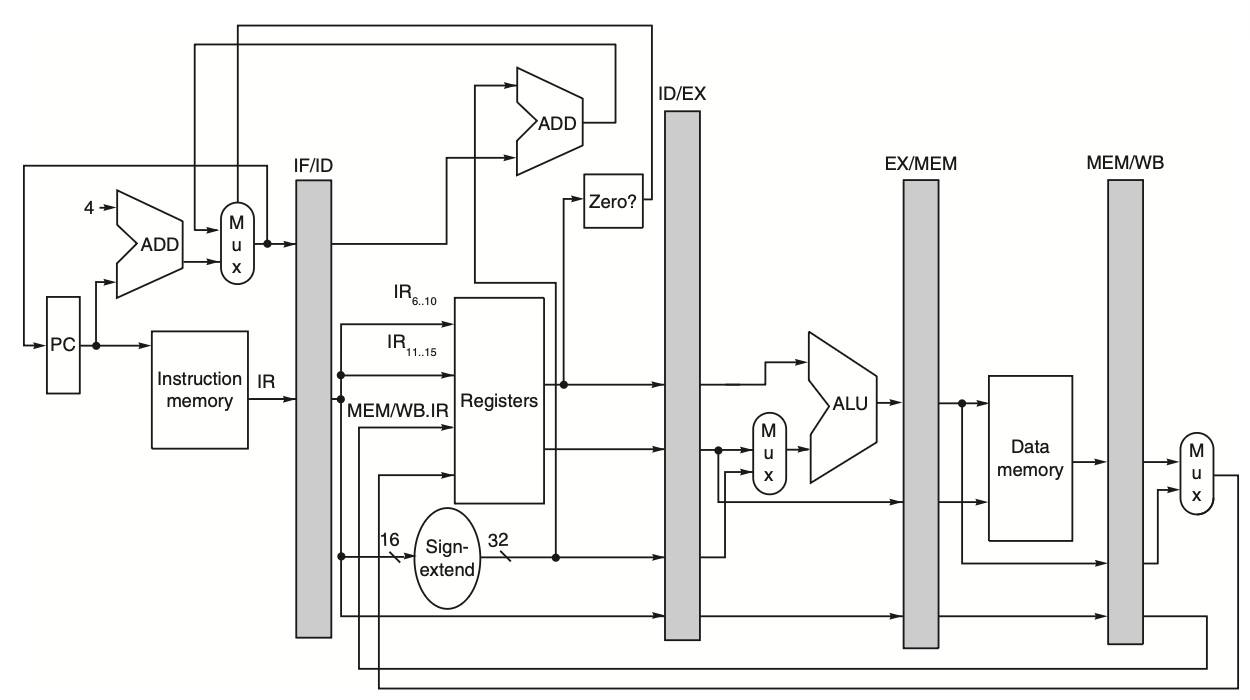
\includegraphics[width=\linewidth]{assets/figures/diag-46.png}
\diagramsource{H\&P Fig.~C.28, \hppage{C}{42} (image supplied by the note-taker; zero test and branch-target adder moved into ID); cf.\ \nolinkurl{03-pipelining-lecture.pdf}, slide 61 (``Pipelined MIPS Datapath'')}
\end{minipage}
\end{center}
{\small \emph{Modified MIPS pipeline: conditional branch completed in the ID
stage; branch penalty $=2-1=1$ cycle.}}

\paragraph{Branch stall impact}

\begin{eg}[Impact of a 3-cycle branch stall]
If CPI $=1$ and $30\%$ of instructions are branches with a 3-cycle stall:
new CPI $= 1 + 0.30\times3 = 1.9$ -- almost double! Reducing the penalty to
1 cycle (MIPS solution above) is therefore very valuable.
\end{eg}

\subsubsection{Four Branch Hazard Alternatives}
\label{sec:branch-alternatives}

\paragraph{\#1: Stall until branch direction is clear}
Simplest, but wastes cycles as shown above.

\paragraph{\#2: Predict Branch Not Taken (most common)}
\begin{itemize}
  \item Execute successor instructions in sequence.
  \item ``Squash'' instructions in the pipeline if the branch is actually
  taken.
  \item Advantage: late pipeline state update (nothing irrevocable has
  happened yet).
  \item About $47\%$ of MIPS branches are not taken on average.
  \item $PC+4$ is already calculated, so it is used to fetch the next
  instruction.
\end{itemize}

\textbf{Predict-not-taken timing (branch penalty $=1$ cycle, ID-stage resolution).}
\begin{lstlisting}[caption={Not taken (no stall)}]
                c1    c2    c3    c4    c5    c6    c7
Untaken branch  IF    ID    EX    MEM   WB
Instr i+1             IF    ID    EX    MEM   WB
Instr i+2                   IF    ID    EX    MEM   WB
\end{lstlisting}
\begin{lstlisting}[caption={Taken (1 idle cycle)}]
                c1    c2    c3    c4    c5    c6    c7
Taken branch    IF    ID    EX    MEM   WB
Instr i+1             IF    idle  idle  idle  idle
Branch target               IF    ID    EX    MEM   WB
\end{lstlisting}
\begin{prop}[Branch stall cycles]
\[
  \text{Pipeline stall cycles from branches} = \text{frequency of taken branches} \times \text{branch penalty}
\]
\end{prop}

\paragraph{\#3: Predict Branch Taken}
\begin{itemize}
  \item About $53\%$ of MIPS branches are taken on average.
  \item But (in the basic MIPS pipeline) the branch target address hasn't
  been calculated yet, so MIPS still incurs a 1-cycle branch penalty even
  with this scheme (other machines that know the branch target before the
  outcome can benefit more).
\end{itemize}

\paragraph{\#4: Delayed Branch}

\begin{definition}[Delayed branch]
Define the branch to take place \emph{after} a following instruction:
\begin{lstlisting}
branch instruction
  sequential successor 1  <- branch delay slot(s)
  ...
  sequential successor n
branch target if taken
\end{lstlisting}
A single delay slot suffices for proper branch-decision and branch-target
computation in a 5-stage pipeline. \textbf{MIPS uses this.}\HPA[25]{C}{\S C.2, Figure~C.14}{23}
\end{definition}

\textbf{Delayed branch timing (no stalls, whether or not taken).}
\begin{lstlisting}
                c1    c2    c3    c4    c5    c6    c7
Untaken branch  IF    ID    EX    MEM   WB
Delay slot i+1        IF    ID    EX    MEM   WB
Instr i+2                   IF    ID    EX    MEM   WB
\end{lstlisting}
\begin{lstlisting}
                c1    c2    c3    c4    c5    c6    c7
Taken branch    IF    ID    EX    MEM   WB
Delay slot i+1        IF    ID    EX    MEM   WB
Branch target               IF    ID    EX    MEM   WB
\end{lstlisting}
The behaviour of the delay-slot instruction is the same whether or not the
branch is taken.

\paragraph{Scheduling branch delay slots}

\begin{center}
\begin{tabular}{@{}p{4.6cm}p{4.6cm}p{4.6cm}@{}}
\toprule
\textbf{A. From before branch} & \textbf{B. From branch target} & \textbf{C. From fall-through} \\
\midrule
\begin{lstlisting}
add $1,$2,$3
if $2=0 then
  (delay slot)
\end{lstlisting}
becomes
\begin{lstlisting}
if $2=0 then
  add $1,$2,$3
\end{lstlisting}
&
\begin{lstlisting}
sub $4,$5,$6
add $1,$2,$3
if $1=0 then
  (delay slot)
\end{lstlisting}
becomes
\begin{lstlisting}
sub $4,$5,$6
add $1,$2,$3
if $1=0 then
  sub $4,$5,$6
\end{lstlisting}
&
\begin{lstlisting}
add $1,$2,$3
if $1=0 then
  (delay slot)
or  $7,$8,$9
sub $4,$5,$6
\end{lstlisting}
becomes
\begin{lstlisting}
add $1,$2,$3
if $1=0 then
  or $7,$8,$9
sub $4,$5,$6
\end{lstlisting}
\\
\bottomrule
\end{tabular}
\end{center}

\begin{itemize}
  \item \textbf{A} is the best choice: it always improves performance
  (fills the delay slot without duplicating any instruction, reducing
  instruction count). The branch must not depend on the rescheduled
  instruction.
  \item In \textbf{B}, the moved instruction may need to be \emph{copied},
  increasing instruction count; it must be safe to execute even if the
  branch is not taken.
  \item In \textbf{C}, the instruction must be safe to execute even if the
  branch \emph{is} taken.
\end{itemize}

\textbf{Three cases for choosing the delay-slot instruction.}
\begin{description}[leftmargin=2.2cm,style=nextline]
  \item[A -- independent instruction from before the branch (\emph{common})]
  Always improves performance when used; the branch must not depend on the
  rescheduled instruction.
  \item[B -- instruction from the branch target] Improves performance if
  the branch is taken; may require duplication; must be safe if the branch
  is \emph{not} taken.
  \item[C -- instruction from the fall-through stream] Improves performance
  if the branch is \emph{not} taken; must be safe if the branch \emph{is}
  taken.
\end{description}
\begin{remark}
The usability of cases B and C is improved by using a \textbf{canceling
(nullifying) branch}.
\end{remark}

\paragraph{Delayed branch: compiler effectiveness}

\begin{itemize}
  \item Fills about $60\%$ of branch delay slots.
  \item About $80\%$ of instructions placed in delay slots are useful.
  \item $\Rightarrow$ about $50\%$ ($60\%\times80\%$) of slots are
  \emph{usefully} filled.
\end{itemize}
\begin{remark}
\textbf{Downside:} as processors move to deeper pipelines and multiple
issue, the branch delay grows and more than one delay slot is needed.
Delayed branching has lost popularity relative to more flexible (but more
expensive) dynamic approaches, since growth in available transistors has
made dynamic branch prediction relatively cheaper.
\end{remark}

\paragraph{Evaluating branch alternatives}

\begin{prop}[Pipeline speedup with branches]
\[
  \text{Pipeline speedup} = \frac{\text{Pipeline depth}}{1+\text{Branch frequency} \times \text{Branch penalty}}
\]\HPA[27]{C}{\S C.2, Performance of Branch Schemes}{25}
\end{prop}

\begin{eg}[Comparing branch schemes]
Assume $4\%$ unconditional branches, $6\%$ untaken conditional branches and
$10\%$ taken conditional branches.

\begin{center}
\small
\begin{tabular}{@{}lcccc@{}}
\toprule
Scheme & Branch penalty & CPI & vs.\ unpipelined & vs.\ stall \\
\midrule
Stall pipeline    & 3                         & 1.60 & 3.1 & 1.00 \\
Predict not taken & $1{\times}0.04+3{\times}0.10$ & 1.34 & 3.7 & 1.19 \\
Predict taken     & $1{\times}0.14+2{\times}0.06$ & 1.26 & 4.0 & 1.29 \\
Delayed branch    & 0.5                       & 1.10 & 4.5 & 1.45 \\
\bottomrule
\end{tabular}
\end{center}

\end{eg}

\paragraph{Pipeline performance example}

\begin{eg}[CPI of a realistic mix]
MIPS instruction mix:

\begin{center}
\begin{tabular}{@{}lp{9.5cm}@{}}
\toprule
Type & Frequency \\
\midrule
Arith/Logic & 40\% \\
Load        & 30\% (of which 25\% are immediately followed by an instruction using the loaded value) \\
Store       & 10\% \\
Branch      & 20\% (of which 45\% are taken) \\
\bottomrule
\end{tabular}
\end{center}

With forwarding and branch-address calculation in the ID stage, using a
branch-not-taken scheme (branch penalty $=1$ cycle):
\[
  \mathrm{CPI} = 1 + \underbrace{0.3\times0.25\times1}_{\text{load-use stalls}} + \underbrace{0.2\times0.45\times1}_{\text{branch stalls}} = 1 + 0.075 + 0.09 = 1.165
\]
\end{eg}

% =============================================================================
\subsection{Textbook Exercises}
\label{sec:pipe-tbx}

\begin{tbexercise}[C]{C.1}{82}{\S C.2, \hppages{C}{11}{27}}
\begin{lstlisting}
Loop: LD    R1,0(R2)    ; load R1 from address 0+R2
      DADDI R1,R1,#1    ; R1 = R1+1
      SD    R1,0(R2)    ; store R1 at address 0+R2
      DADDI R2,R2,#4    ; R2 = R2+4
      DSUB  R4,R3,R2    ; R4 = R3-R2
      BNEZ  R4,Loop     ; branch to Loop if R4 != 0
\end{lstlisting}
Initially R3 $=$ R2 $+$ 396. (a) List all data dependences (register, source,
destination). (b) Draw the timing on the 5-stage pipeline without forwarding (a
register written and read in the same cycle is forwarded through the register file),
branches handled by flushing; how many cycles does the loop take? (c) With full
forwarding, predict not taken. (d) With full forwarding, predict taken. (e) A 10-stage
pipeline splits every stage in two; forwarding goes from the end of a pair of stages
to the start of the pair that needs it; predict taken. (f) The longest 5-stage stage
takes 0.8 ns and the pipeline register 0.1 ns: the cycle time of the 5- and 10-stage
machines? (g) The CPI of the loop on each, and the average instruction time.
\end{tbexercise}

\begin{tbexercise}[C]{C.2}{83}{\S C.2 (branch penalties), \hppages{C}{21}{27}}
Conditional branches are 15\% of instructions (60\% taken), jumps and calls 1\%.
(a) In a 4-deep pipeline, unconditional branches resolve at the end of cycle 2 and
conditional ones at the end of cycle 3; only the first stage is independent of the
branch outcome. How much faster would the machine be without branch hazards? (b) The
same for a 15-deep pipeline resolving at the end of cycles 5 and 10.
\end{tbexercise}

\begin{tbexercise}[C]{C.3}{83}{\S C.1--C.2, \hppages{C}{10}{13}}
A single-cycle machine has a 7 ns clock. Split into stages: IF 1, ID 1.5, EX 1, MEM 2,
WB 1.5 ns; pipeline register delay 0.1 ns. (a) Clock cycle of the 5-stage pipeline?
(b) CPI with a stall every 4 instructions? (c) Speedup over the single-cycle machine?
(d) Speedup with infinitely many stages?
\end{tbexercise}

\begin{tbexercise}[C]{C.4}{84}{\S C.2, \hppages{C}{21}{23}}
Resolving branches in ID instead of MEM reduces control stalls but can create a new
data hazard. Write a short code snippet where computing the branch in ID causes a
data hazard even with forwarding.
\end{tbexercise}

